\documentclass[10pt,a4paper]{article}

% -----------------------------------------------------------------------------
% TIW-DSM Deliverable 3 - Final Report (LaTeX source)
% Machine Learning course, Fall 2026
% Compile:  python scripts/make_report_assets.py --runs obs=runs/obs tiw=runs/tiw
%           cd report && latexmk -pdf main.tex
% Every experimental number is read from generated/numbers.tex (written by the
% evaluation scripts). Missing results print as a red [pending] marker.
% -----------------------------------------------------------------------------

\usepackage[a4paper,left=18mm,right=18mm,top=17mm,bottom=20mm]{geometry}
\usepackage[T1]{fontenc}
\usepackage[utf8]{inputenc}
\usepackage{lmodern}
\usepackage{microtype}
\usepackage{graphicx}
\usepackage{booktabs}
\usepackage{tabularx}
\usepackage{array}
\usepackage{multirow}
\usepackage{enumitem}
\usepackage{amsmath,amssymb,amsthm}
\usepackage{xcolor}
\usepackage{caption}
\usepackage{fancyhdr}
\usepackage{listings}
\usepackage{tikz}
\usetikzlibrary{arrows.meta,positioning}
\usepackage[ruled,vlined,linesnumbered]{algorithm2e}
\usepackage{hyperref}
\usepackage{xurl}
\usepackage{float}

\definecolor{Navy}{HTML}{17365D}
\definecolor{Blue}{HTML}{2F75B5}
\definecolor{Teal}{HTML}{18A999}
\definecolor{PaleBlue}{HTML}{EAF2F8}
\definecolor{Grey}{HTML}{5F6B75}
\definecolor{Pend}{HTML}{C0392B}
\definecolor{TodoBg}{HTML}{FFF4D6}
\definecolor{TodoFr}{HTML}{E8871E}
\definecolor{RuleGreyC}{HTML}{C5D3E0}

\hypersetup{colorlinks=true,linkcolor=Navy,citecolor=Blue,urlcolor=Blue,
  pdftitle={TIW-DSM Deliverable 3 Final Report},
  pdfauthor={Syed Zain Afaq, Shaheer Ahmed Farooqui, Huzaifa}}

\setlength{\parindent}{0pt}
\setlength{\parskip}{4pt}
\setlength{\tabcolsep}{5pt}
\renewcommand{\arraystretch}{1.13}
\raggedbottom
\newcolumntype{Y}{>{\raggedright\arraybackslash}X}

\makeatletter
\renewcommand\section{\@startsection{section}{1}{\z@}{1.2ex \@plus .2ex \@minus .1ex}{0.5ex \@plus .1ex}{\normalfont\Large\bfseries\color{Navy}}}
\renewcommand\subsection{\@startsection{subsection}{2}{\z@}{0.9ex \@plus .2ex \@minus .1ex}{0.3ex \@plus .1ex}{\normalfont\normalsize\bfseries\color{Blue}}}
\renewcommand\subsubsection{\@startsection{subsubsection}{3}{\z@}{0.6ex}{0.2ex}{\normalfont\normalsize\itshape\color{Navy}}}
\makeatother

\captionsetup{font={small},labelfont={bf,color=Navy},justification=centering,skip=3pt}
\pagestyle{fancy}\fancyhf{}
\renewcommand{\headrulewidth}{0pt}\renewcommand{\footrulewidth}{0.4pt}
\fancyfoot[L]{\footnotesize\color{Grey}TIW-DSM Final Report -- Deliverable 3}
\fancyfoot[R]{\footnotesize\color{Grey}Page \thepage}
\fancypagestyle{plain}{\fancyhf{}\renewcommand{\headrulewidth}{0pt}\renewcommand{\footrulewidth}{0pt}}

\lstset{basicstyle=\ttfamily\footnotesize,breaklines=true,frame=single,rulecolor=\color{RuleGreyC},
  backgroundcolor=\color{PaleBlue},columns=fullflexible,keepspaces=true,showstringspaces=false}

\newtheorem{theorem}{Theorem}
\newcommand{\Dbias}{\mathcal{D}_{\mathrm{bias}}}
\newcommand{\Dref}{\mathcal{D}_{\mathrm{ref}}}
\newcommand{\Dobs}{\mathcal{D}_{\mathrm{obs}}}
\newcommand{\pdata}{p_{\mathrm{data}}}
\newcommand{\pbias}{p_{\mathrm{bias}}}
\newcommand{\pobs}{p_{\mathrm{obs}}}
\newcommand{\callout}[1]{\begin{center}\fcolorbox{Blue}{PaleBlue}{\parbox{0.93\linewidth}{\color{Navy}#1}}\end{center}}
\newcommand{\pending}{\textcolor{Pend}{\textbf{[pending]}}}
\newcommand{\todobox}[1]{\begin{center}\fcolorbox{TodoFr}{TodoBg}{\parbox{0.93\linewidth}{\small\textbf{\color{TodoFr}FINALISE AFTER RESULTS:} #1}}\end{center}}
\newcommand{\pendingfig}[2][0.32\textheight]{\fcolorbox{Pend}{white}{\parbox[c][#1][c]{0.9\linewidth}{\centering\color{Pend}\textbf{[pending figure]}\\[2pt]\small #2}}}
\makeatletter\newcommand{\rowsfile}[1]{\@@input generated/#1.tex }\makeatother
\newcommand{\fig}[3][\linewidth]{\IfFileExists{figures/#2}{\includegraphics[width=#1]{figures/#2}}{\pendingfig{#3}}}

% ---- links (replace before submission) --------------------------------------
\newcommand{\repoURL}{\url{https://github.com/shaheer-geeksofkolachi/tiw-dsm-repro}}
\newcommand{\appURL}{\url{https://tiwdsm-cifar10-demo.streamlit.app}}
\newcommand{\weightsURL}{\url{https://github.com/shaheer-geeksofkolachi/tiw-dsm-repro/tree/main/checkpoints/deploy}}

% ---- experimental numbers ----------------------------------------------------
\input{generated/defaults.tex}
\IfFileExists{generated/numbers.tex}{\input{generated/numbers.tex}}{}

\begin{document}

% ================================ COVER ======================================
\thispagestyle{plain}
\vspace*{10mm}
\begin{center}
  {\large\color{Grey}MACHINE LEARNING -- FALL 2026\par}
  \vspace{6mm}
  {\fontsize{23}{28}\selectfont\bfseries\color{Navy}Deliverable 3: Final Report\par}
  \vspace{5mm}
  {\large\color{Grey}Reproduction and Deployment of\\[1mm]\textit{Training Unbiased Diffusion Models From Biased Dataset}\par}
  \vspace{2mm}
  {\normalsize\color{Grey}Time-dependent Importance Reweighting (TIW-DSM) on CIFAR-10 Long-Tail with 5\% reference data\par}
\end{center}
\vspace{7mm}
\begin{center}
\begin{tabularx}{0.88\textwidth}{>{\color{Grey}\small}p{36mm}Y}
\toprule
Selected paper & Kim et al., ICLR 2024 \cite{kim2024tiwdsm} \\ \midrule
Area & Generative models -- diffusion models, dataset bias \\ \midrule
Project setting & CIFAR-10 LT, $|\Dbias|=10{,}000$ (100.75:1 imbalance), $|\Dref|=500$ \\ \midrule
Prepared by & Syed Zain Afaq -- 36234 \\
            & Shaheer Ahmed Farooqui -- 19722 \\
            & Huzaifa -- 19193 \\ \midrule
Submission & Final Report, Source Code \& Trained Model (hard freeze 25 Nov 2026, 23:55) \\ \midrule
Date & 25 November 2026 \\
\bottomrule
\end{tabularx}
\end{center}
\vspace{5mm}
\subsection*{Project artifacts (view and download without permission requests)}
\begin{center}
\begin{tabularx}{0.93\textwidth}{>{\bfseries\small}p{40mm}Y}
\toprule
Source code (GitHub) & \repoURL \\
Trained weights & \weightsURL\ \ (\texttt{tiw\_dsm.pt}, \texttt{dsm\_obs.pt}; also in the Kaggle output of \texttt{tiw-dsm-eval}) \\
Training / evaluation runs & \url{https://www.kaggle.com/code/shaheerfarooqui19722/tiw-dsm-train}, \url{https://www.kaggle.com/code/shaheerfarooqui19722/tiw-dsm-eval} \\
Run everything & \texttt{README.md} and \texttt{notebooks/run\_on\_kaggle.ipynb} in the repository \\
Live deployed app & \appURL\ \ (Streamlit Community Cloud, CPU; Section~\ref{sec:deploy}) \\
Run the app locally & \texttt{streamlit run app/streamlit\_app.py} \\
LaTeX source & \texttt{report/main.tex}, \texttt{report/references.bib} (bonus; Deliverable 2 was also in \LaTeX) \\
\bottomrule
\end{tabularx}
\end{center}
\callout{\textbf{Summary.} We re-implemented TIW-DSM in our own PyTorch code (time-dependent discriminator, reweighted and score-corrected objective, EDM sampler, evaluation suite, Streamlit app) and trained DSM(obs) and TIW-DSM on the authors' exact CIFAR-10 LT / 5\% files on free Kaggle GPUs, comparing both at the same 3.51M training images. \textbf{The debiasing claim reproduced:} the share of generated tail-class images rose from \resTailobs\% (DSM(obs)) to \resTailtiw\% (target 50\%), and the paper's Eq.~51 bias fell from \resBiasobs{} to \resBiastiw{} (\resBiasRed\% lower). \textbf{The FID improvement did not:} under our reduced compute TIW-DSM scored FID \resFIDtiw{} vs.\ \resFIDobs{} (paper: 11.51 vs.\ 12.99), with higher precision but lower recall. Our diagnostics point to an over-confident discriminator that gives almost zero weight to biased images at low noise. The additional experiment shows TIW-DSM keeps its lower bias at every sampling budget of 17 network evaluations or more.}

\newpage
\tableofcontents
\listoffigures
\listoftables
\newpage

% ============================================================================
\section{Introduction and Problem Statement}\label{sec:intro}
% ============================================================================
A generative model learns whatever distribution its training data come from. If the data were collected unevenly, the model faithfully reproduces that unevenness. For diffusion models this is a practical problem. Large image collections are shaped by where, how and by whom they were gathered \cite{torralba2011datasetbias}, so a model can produce realistic images while still getting the \emph{proportions} of what it generates wrong.

Kim et al.\ \cite{kim2024tiwdsm} study the following setting. We have a large dataset $\Dbias$ drawn from an unknown biased distribution $\pbias$, and a small dataset $\Dref$ drawn from the distribution we actually want, $\pdata$. We know which set each image came from, but nothing else: no attribute labels and no description of the bias.

\callout{\textbf{Problem statement.} Given a large biased set $\Dbias$ and a small unbiased reference set $\Dref$ ($|\Dref| \ll |\Dbias|$), train a diffusion model whose samples follow $\pdata$. Use the variety of $\Dbias$ without inheriting its bias, and without overfitting to the few images in $\Dref$.}

In our instance, $\Dbias$ is the authors' long-tailed CIFAR-10 split. It has 10{,}000 images with class counts falling from 4{,}030 (airplane) to 40 (truck), so airplanes and automobiles make up 64.5\% of it. $\Dref$ is a random 5\% reference set of 500 images that is close to class-balanced. The target is the balanced CIFAR-10 training distribution \cite{krizhevsky2009cifar}.

\textbf{What this project delivers.}
\begin{itemize}[leftmargin=5mm,itemsep=1pt,topsep=1pt]
  \item A from-scratch implementation of TIW-DSM and its baselines. The objective is derived in EDM's denoiser form (Section~\ref{sec:method}) and checked on the paper's 2-D example (Section~\ref{sec:verify}).
  \item A reduced-compute reproduction on the paper's exact CIFAR-10 LT / 5\% files, with every deviation listed and its expected effect stated (Table~\ref{tab:config}).
  \item An evaluation that matches the paper's protocol: FID against the full unbiased training set, the paper's Eq.~51 bias metric with a VGG13-BN classifier, plus precision/recall and class shares (Section~\ref{sec:results}).
  \item An additional experiment on the sampling budget (Section~\ref{sec:extra}), and a deployed Streamlit application (Section~\ref{sec:deploy}).
\end{itemize}

% ============================================================================
\section{Literature Review and Background}\label{sec:lit}
% ============================================================================
\textit{Carried over from Deliverable 2 and refined; changes are listed in Appendix~\ref{app:revisions}.}

\subsection{Dataset bias in generative models}
Dataset bias is a long-standing problem in vision. Each benchmark reflects choices about where and how images were collected \cite{torralba2011datasetbias}. Discriminative models inherit it as poor generalisation. Generative models inherit it more directly, because their output distribution \emph{is} the learned data distribution. In our data, a standard model sees 100 airplanes for every truck, and it is expected to generate them at roughly that rate. Visual quality alone cannot reveal this. One has to measure the distribution of generated content.

\subsection{Diffusion models and denoising score matching}
Diffusion models gradually corrupt data with Gaussian noise and learn to reverse the corruption \cite{ho2020ddpm,song2021sde}. The reverse process needs the \emph{score} $\nabla_{\mathbf{x}_t}\log p^t(\mathbf{x}_t)$ at every noise level. The score is unknown, so denoising score matching (DSM) \cite{vincent2011dsm} trains a network $\mathbf{s}_\theta$ to match the tractable conditional score $\nabla\log p(\mathbf{x}_t|\mathbf{x}_0)$. In expectation, this has the same minimiser as matching the true score:
\begin{equation}
\mathcal{L}_{\mathrm{DSM}}(\theta;p)=\tfrac12\int_0^T\lambda(t)\,\mathbb{E}_{p(\mathbf{x}_0)}\mathbb{E}_{p(\mathbf{x}_t|\mathbf{x}_0)}\big\|\mathbf{s}_\theta(\mathbf{x}_t,t)-\nabla\log p(\mathbf{x}_t|\mathbf{x}_0)\big\|_2^2\,dt .
\end{equation}
Its key weakness for our problem is that DSM learns whatever $p$ the samples come from. Trained on biased data, it learns the biased score. EDM \cite{karras2022edm} re-parameterises the model as a denoiser $D_\theta(\mathbf{x};\sigma)$ with $\mathbf{s}_\theta=(D_\theta-\mathbf{x})/\sigma^2$, together with preconditioning, a log-normal training-noise distribution and a 2nd-order Heun ODE sampler. Both the official TIW-DSM code and our implementation use this formulation.

\subsection{Approaches before TIW-DSM}
\textbf{DSM(ref): train on $\Dref$ only.} This targets the right distribution, but 500 images are far too few for a diffusion model. The model memorises and loses diversity \cite{kim2024tiwdsm}. Augmentation helps only partly \cite{karras2020ada}.

\textbf{DSM(obs): train on everything.} Using $\Dobs=\Dbias\cup\Dref$ gives diversity but keeps the bias. The model converges to the observed mixture, not to $\pdata$.

\textbf{Importance reweighting (IW).} If the density ratio $w(\mathbf{x})=\pdata(\mathbf{x})/\pbias(\mathbf{x})$ were known, weighting each biased sample by $w$ would give an unbiased objective. Choi et al.\ \cite{choi2020fair} estimate $w$ with a probabilistic classifier that separates reference from biased samples: if $d(\mathbf{x})=P(\text{ref}\mid\mathbf{x})$ with balanced classes, then $w=d/(1-d)$. Plugged into DSM on clean data, this gives the \emph{IW-DSM} baseline.

\subsection{Density-ratio estimation and the density chasm}
Classifier-based density-ratio estimation \cite{sugiyama2012dre} is accurate only when the two distributions overlap. When they are far apart, for example high-dimensional images with a small reference set, a classifier separates them almost perfectly. Its probabilities then saturate and the implied ratio is badly estimated. This is the \emph{density-chasm} problem \cite{rhodes2020tre}. Telescoping ratio estimation bridges the chasm through intermediate distributions. The diffusion forward process naturally provides such a bridge, and this is the observation TIW-DSM is built on.

\subsection{Positioning of TIW-DSM}
TIW-DSM \cite{kim2024tiwdsm} (i) estimates the ratio between the \emph{perturbed} distributions $\pdata^t/\pbias^t$ at every diffusion time, where they overlap more and the estimate is easier, and (ii) uses it twice: as a sample weight, and through its gradient as a correction to the score. It reuses the time-dependent discriminator design of Discriminator Guidance \cite{kim2023dg}, built on a pretrained ADM encoder \cite{dhariwal2021adm}. In the paper's 2-D experiment, the integrated error of the time-dependent ratio was only 39.1\% of the time-independent error. Table~\ref{tab:paperfid} recalls the reported CIFAR-10 LT results that we try to reproduce.

\begin{table}[H]
\centering
\caption{Reported CIFAR-10 LT FID-50k (lower is better) for different reference-set sizes \cite{kim2024tiwdsm}. Our project targets the 5\% column. These are the \emph{authors'} results.}
\label{tab:paperfid}
\begin{tabular}{lrrrr}
\toprule
Method & 5\% & 10\% & 25\% & 50\% \\ \midrule
DSM(ref) & 16.47 & 11.56 & 10.77 & 5.19 \\
DSM(obs) & 12.99 & 10.75 & 8.45 & 7.35 \\
IW-DSM   & 15.79 & 11.45 & 8.19 & 4.28 \\
\textbf{TIW-DSM} & \textbf{11.51} & \textbf{8.08} & \textbf{5.59} & \textbf{4.06} \\
\bottomrule
\end{tabular}
\end{table}

% ============================================================================
\section{Paper Methodology}\label{sec:method}
% ============================================================================
This section explains the method in our own words and derives the exact form we implement.

\subsection{Why make the density ratio time-dependent?}
The forward diffusion maps both $\pbias$ and $\pdata$ through the same Gaussian blurring kernel, giving $\pbias^t$ and $\pdata^t$. As $t$ grows the two become smoother and overlap more, and at $t=T$ both are the same Gaussian. A classifier that sees noisy images therefore faces an easier problem at larger $t$. Its probabilities are less saturated and the ratio $w^t=\pdata^t/\pbias^t$ is better calibrated. The diffusion model needs the score at \emph{every} $t$ anyway, so it is natural to use the ratio at the same $t$ instead of the clean-data ratio $w^0$.

\subsection{Time-dependent discriminator}
A discriminator $d_\phi(\mathbf{x}_t,t)$ is trained with binary cross-entropy to tell noisy reference samples (label 1) from noisy biased samples (label 0), drawing both in equal numbers at random diffusion times:
\begin{equation}
\mathcal{L}_{\mathrm{disc}}(\phi)=-\mathbb{E}_t\Big[\mathbb{E}_{\pdata^t}\log d_\phi(\mathbf{x}_t,t)+\mathbb{E}_{\pbias^t}\log\big(1-d_\phi(\mathbf{x}_t,t)\big)\Big].
\end{equation}
The optimum is $d^*=\pdata^t/(\pdata^t+\pbias^t)$, hence $w^t=d^*/(1-d^*)$.

\subsection{The TIW-DSM objective}
TIW-DSM weights the DSM loss by $w^t(\mathbf{x}_t)$ and also shifts the regression target by $\nabla\log w^t$:
\begin{equation}\label{eq:tiw}
\mathcal{L}_{\mathrm{TIW}}=\tfrac12\int_0^T\lambda(t)\,\mathbb{E}_{\pbias(\mathbf{x}_0)}\mathbb{E}_{p(\mathbf{x}_t|\mathbf{x}_0)}
\Big[w^t(\mathbf{x}_t)\big\|\mathbf{s}_\theta(\mathbf{x}_t,t)-\nabla\log p(\mathbf{x}_t|\mathbf{x}_0)-\nabla\log w^t(\mathbf{x}_t)\big\|_2^2\Big]dt .
\end{equation}
\begin{theorem}[Kim et al.\ \cite{kim2024tiwdsm}, Thm.~1]
With the exact ratio, $\mathcal{L}_{\mathrm{TIW}}(\theta;\pbias,w^t)=\mathcal{L}_{\mathrm{SM}}(\theta;\pdata)+C$, where $C$ does not depend on $\theta$. The minimiser is therefore the score of the \emph{unbiased} distribution.
\end{theorem}
\textbf{Intuition (our sketch).} Two facts make this work. First, $w^t\pbias^t=\pdata^t$, so the weight turns an expectation under the biased marginal into one under the target marginal. Second, $\nabla\log\pdata^t=\nabla\log\pbias^t+\nabla\log w^t$, and DSM on biased samples already supplies $\nabla\log\pbias^t$ in expectation. Adding $\nabla\log w^t$ to the target supplies the missing part. Expanding the square and taking the conditional expectation over $\mathbf{x}_0$ given $\mathbf{x}_t$ turns the objective into score matching against $\nabla\log\pdata^t$ under $\pdata^t$.

\subsection{Why both terms are needed}\label{sec:whyboth}
This point became clear to us during implementation and is easy to miss. Look at the per-$\mathbf{x}_t$ minimiser of a weighted DSM loss $\mathbb{E}[\,w(\mathbf{x}_t)\|\mathbf{s}-\mathbf{y}\|^2]$ with $\mathbf{y}=\nabla\log p(\mathbf{x}_t|\mathbf{x}_0)$. Because the weight depends only on $\mathbf{x}_t$, it factors out of the conditional expectation, and the minimiser is still $\mathbb{E}[\mathbf{y}\mid\mathbf{x}_t]=\nabla\log\pbias^t$.
\begin{itemize}[leftmargin=5mm,itemsep=1pt,topsep=1pt]
\item \textbf{Weighting only (W):} with infinite capacity it still learns the \emph{biased} score. A time-dependent weight only redistributes model capacity and gradient variance across $\mathbf{x}_t$.
\item \textbf{Correction only (C):} the minimiser is $\nabla\log\pbias^t+\nabla\log w^t=\nabla\log\pdata^t$, which is consistent. However, every region keeps its biased share of training signal.
\item \textbf{W + C (TIW-DSM):} consistent, and it also spends model capacity in proportion to the target density.
\end{itemize}
This matches the paper's ablation at 5\% (Table~4 in \cite{kim2024tiwdsm}): none 12.99, W only 13.27, C only 11.62, both 11.51 FID. It also matches our 2-D check (Section~\ref{sec:verify}).

\subsection{Practical form used in the paper and in our code}\label{sec:practical}
\textbf{Training on $\Dobs$.} The authors train the score model on $\Dobs=\Dbias\cup\Dref$, with $\Dref$ repeated so that the two sources are 1:1. The sampling distribution is then $\pobs=\tfrac12\pbias+\tfrac12\pdata$, and the required ratio becomes (paper Eq.~36)
\begin{equation}
\tilde w^t=\frac{\pdata^t}{\pobs^t}=\frac{2w^t}{1+w^t}=2\,d_\phi(\mathbf{x}_t,t),\qquad \nabla\log\tilde w^t=\nabla\log d_\phi(\mathbf{x}_t,t).
\end{equation}
The weight is bounded in $(0,2)$, which keeps training stable. The weight is not $d/(1-d)$, which can explode.

\textbf{EDM denoiser form (our derivation).} With $\mathbf{x}=\mathbf{y}+\sigma\mathbf{n}$, $\mathbf{s}_\theta=(D_\theta-\mathbf{x})/\sigma^2$ and $\nabla\log p(\mathbf{x}|\mathbf{y})=(\mathbf{y}-\mathbf{x})/\sigma^2$, the TIW integrand becomes
\begin{equation}\label{eq:edmtiw}
\frac{\tilde w}{\sigma^4}\Big\|D_\theta(\mathbf{x};\sigma)-\big(\mathbf{y}+\sigma^2\,\nabla_{\mathbf{x}}\log d_\phi(\mathbf{x},\sigma)\big)\Big\|_2^2 .
\end{equation}
So TIW-DSM is ordinary EDM training with a \emph{per-sample weight} $2d_\phi$ and a \emph{shifted target} $\mathbf{y}+\sigma^2\nabla\log d_\phi$. We keep EDM's weighting $\lambda(\sigma)=(\sigma^2+\sigma_d^2)/(\sigma\sigma_d)^2$ (the time weighting is a free choice and does not affect consistency). The discriminator lives in VP space, so an EDM sample is converted with $\alpha=1/\sqrt{1+\sigma^2}$, $\mathbf{x}_{\mathrm{VP}}=\alpha\mathbf{x}$, and the VP time $\tau$ that solves $\alpha(\tau)=\alpha$. The gradient is taken with respect to the EDM-space $\mathbf{x}$, so the chain-rule factor $\alpha$ is included automatically.

\textbf{Inference.} The discriminator is used \emph{only during training}. At sampling time TIW-DSM is a plain diffusion model, so it adds no inference cost.

\begin{algorithm}[H]
\caption{TIW-DSM training as implemented (two stages)}\label{alg:tiw}
\SetKwInOut{Input}{Input}
\Input{$\Dbias$, $\Dref$, frozen ADM feature extractor, denoiser $D_\theta$}
\tcp{Stage 1: time-dependent discriminator}
\For{$k=1,\dots,10{,}000$}{
  draw $B$ images from $\Dref$ (label 1) and $B$ from $\Dbias$ (label 0); draw $\tau$ by importance sampling\;
  $\mathbf{x}_\tau=\alpha(\tau)\mathbf{x}_0+\sqrt{1-\alpha(\tau)^2}\,\mathbf{z}$; \ update the head $\phi$ with BCE on $d_\phi(\mathbf{x}_\tau,\tau)$\;
}
freeze $\phi$\;
\tcp{Stage 2: score model on $\Dobs=\Dbias\cup 20\times\Dref$}
\While{trained images $<$ budget}{
  $\mathbf{y}\sim\Dobs$ (random x-flip), $\ln\sigma\sim\mathcal{N}(-1.2,1.2^2)$, $\mathbf{x}=\mathbf{y}+\sigma\mathbf{n}$\;
  $d=\mathrm{clip}(d_\phi(\alpha\mathbf{x},\tau(\sigma)),10^{-5},1-10^{-5})$, \ $\mathbf{g}=\nabla_{\mathbf{x}}\log d$ \tcp*{no gradient to $\phi$}
  $\mathcal{L}=\lambda(\sigma)\,2d\,\big\|D_\theta(\mathbf{x};\sigma)-(\mathbf{y}+\sigma^2\mathbf{g})\big\|^2$; \ Adam step on $\theta$; EMA update\;
}
\end{algorithm}

% ============================================================================
\section{Implementation Details}\label{sec:impl}
% ============================================================================
\subsection{Code structure}
The code is a small Python package (\texttt{tiwdsm/}) plus scripts, organised so that each stage of the pipeline can be run and verified separately:
\begin{center}
\small
\begin{tabularx}{\textwidth}{>{\ttfamily}p{44mm}Y}
\toprule
tiwdsm/data.py & loads the official NPZ arrays, builds $\Dobs$ (bias + 20$\times$ ref), $[-1,1]$ normalisation, x-flip \\
tiwdsm/unet.py & compact DDPM++-style U-Net (presets \texttt{tiny/small/base}) \\
tiwdsm/edm.py & EDM preconditioning, $\sigma$ sampling, loss weight, Heun/Euler sampler, EMA \\
tiwdsm/vpsde.py & EDM $\sigma$ $\leftrightarrow$ VP time, importance time sampling \\
tiwdsm/discriminator.py & ADM-encoder discriminator, $\tilde w=2d$, $\nabla\log d$, IW clean weight \\
tiwdsm/losses.py & DSM(obs/ref), IW-DSM, TIW-DSM and the W-only / C-only ablations (Eq.~\ref{eq:edmtiw}) \\
tiwdsm/metrics.py & FID, precision/recall, Eq.~51 bias, class-share metrics \\
scripts/ & \texttt{prepare\_data}, \texttt{train\_discriminator}, \texttt{train\_score}, \texttt{evaluate}, \texttt{steps\_experiment}, \texttt{toy\_2d}, \texttt{make\_report\_assets} \\
app/streamlit\_app.py & deployment \\
\bottomrule
\end{tabularx}
\end{center}

\subsection{Architecture}
\textbf{Score network.} An EDM-preconditioned U-Net that we wrote ourselves, following the DDPM++ design: residual blocks with GroupNorm/SiLU, an additive noise embedding from a positional encoding of $c_{\mathrm{noise}}=\tfrac14\ln\sigma$ through a 2-layer MLP, self-attention at $16\times16$ and in the bottleneck, $\sqrt{1/2}$ skip scaling, zero-initialised output layers and dropout 0.13. Our default \texttt{small} preset (64 base channels, multipliers 1-2-2-2, 2 blocks per level) has \resParams M parameters. The paper's DDPM++ has $\approx$56M; our \texttt{base} preset reproduces that size (53.6M) if more compute is available.

\textbf{Discriminator.} Same architecture as the paper: a \emph{frozen} pretrained ADM classifier encoder (the authors' \texttt{32x32\_classifier.pt}, 47.8M parameters) maps the noisy image to $8\times8\times512$ features. A shallow ADM encoder head (depth 2, width 128, attention pooling, 2.9M trainable parameters) outputs a logit. Time enters both networks through their timestep embeddings ($999\tau$). A small from-scratch CNN backbone is provided as a documented fallback.

\subsection{Training configuration: original vs.\ reproduced}
\begin{table}[H]
\centering
\caption{Original configuration (paper / official command) vs.\ our reproduction, with the expected effect of each deviation.}
\label{tab:config}
\small
\begin{tabularx}{\textwidth}{p{30mm}p{37mm}p{37mm}Y}
\toprule
Item & Original & Ours & Expected effect \\ \midrule
Hardware & 4$\times$ RTX 4090 & 2$\times$ \resStepsDevice{} (free Kaggle; one GPU per model, in parallel) & time only \\
Score network & DDPM++, 56M & DDPM++-style, \resParams M & less capacity; higher absolute FID for \emph{both} methods \\
Batch / lr & 256 / $10^{-3}$, 10 Mimg ramp-up & 256 (TIW: 2$\times$128 micro-batches, GPU memory) / $10^{-3}$, 10 Mimg ramp-up & same effective batch \\
Duration & 11 Mimg & TIW-DSM \resMimgtiw{} Mimg (12-h session limit); DSM(obs) \resMimgobs{} Mimg. \textbf{Compared at 3.51 Mimg} (same checkpoint length for both) & under-trained: higher FID; learning rate only reached 35\% of its peak \\
EMA / dropout & 0.5 Mimg / 0.13 & 0.5 Mimg / 0.13 & same \\
Augmentation & EDM pipeline, $p=0.12$ & horizontal flip only & more memorisation risk on 10.5k unique images \\
Precision & fp32 & fp16 autocast + loss scaling & small numerical noise \\
Discriminator & ADM features + head, 10k it., batch 128+128 & same; lr $3\cdot10^{-4}$ (official script default); \resDiscMinutes{} min on T4 & same \\
Correction term & code: from $\nabla d$ & from $\nabla\log d$ (paper Eq.~10/36) & follows the paper's equation exactly \\
FID & EDM \texttt{fid.py}, 50k vs.\ CIFAR-10 train & \texttt{pytorch-fid} (same TF Inception weights), 50k vs.\ all 50k train images & small constant offset possible \\
Sampler & EDM Heun, 18 steps (35 NFE) & identical & same \\
Bias classifier & VGG13-BN & VGG13-BN (\cite{chenyaofo2021cifar}), test acc.\ \resClfAcc\% & same \\
\bottomrule
\end{tabularx}
\end{table}

All design choices that are not compute-driven follow the official code (checked line by line against the released \texttt{train.py}, \texttt{train\_classifier.py} and \texttt{loss.py}). The only intentional methodological difference is the correction term. The released \texttt{classifier\_lib.get\_weight\_correction} differentiates the discriminator \emph{probability} $d$, whereas the paper's objective uses the gradient of the \emph{log} ratio. We implement the paper's form and list this as an implementation difference rather than a claim about which is better.

\subsection{Environment and dependencies}
\begin{center}\small
\begin{tabularx}{\textwidth}{lY}
\toprule
Language / framework & Python 3.10+, PyTorch $\ge$ 2.1 \cite{paszke2019pytorch} (CUDA for training; CPU works for inference) \\
Training hardware & Kaggle GPU T4 $\times$2 (15 GB each); one 11.3-h session for both models, one 3-h session for evaluation \\
Main packages & numpy, scipy, pillow, pyarrow, gdown, pytorch-fid 0.3.0 \cite{seitzer2020pytorchfid}, matplotlib, streamlit \cite{streamlit} \\
Pinned list & \texttt{requirements.txt} in the repository \\
Seeds & training seed 0; evaluation image $k$ uses noise seed $k$ (identical across models) \\
\bottomrule
\end{tabularx}
\end{center}

\subsection{Code and result attribution}\label{sec:attrib}
\begin{table}[H]
\centering
\caption{Attribution of code and results, following the four categories required by the guidelines.}
\label{tab:attrib}
\small
\begin{tabularx}{\textwidth}{p{40mm}Y}
\toprule
\textbf{(a) Implemented by our team} & U-Net (\texttt{unet.py}); TIW/IW/DSM losses and ablations derived in EDM form (\texttt{losses.py}); discriminator wrapper and ratio/gradient computation (\texttt{discriminator.py}); data pipeline and label recovery (\texttt{data.py}); all training loops (resume, time limit, EMA, AMP); evaluation suite including our own Fréchet distance (robust to new SciPy) and $k$-NN precision/recall; 2-D toy; sampling-step experiment; report-asset generator; Streamlit app. \\ \midrule
\textbf{(b) Adapted from existing code} & EDM formulas (preconditioning, noise distribution, Heun sampler, EMA rule) re-written from \cite{karras2022edm}; VP-SDE conversion and importance time sampling from the official \texttt{classifier\_lib.vpsde} \cite{tiwdsmcode}; discriminator training settings from the official \texttt{train\_classifier.py}. \\ \midrule
\textbf{(c) Reused directly} & \texttt{third\_party/guided\_diffusion/} (OpenAI ADM encoder, copied unchanged from the official repo except one unused import); authors' pretrained \texttt{32x32\_classifier.pt}; authors' data files; \texttt{pytorch-fid} Inception network; pretrained VGG13-BN from \cite{chenyaofo2021cifar}. We did \emph{not} run the official training or sampling scripts. \\ \midrule
\textbf{(d) Authors' vs.\ our results} & Every number from the paper is labelled ``paper'' or ``reported'' (Tables~\ref{tab:paperfid}, \ref{tab:main}). Every other number in Sections~\ref{sec:verify}, \ref{sec:results} and \ref{sec:extra} was produced by our code and is inserted automatically from the JSON result files. \\
\bottomrule
\end{tabularx}
\end{table}

\subsection{Verification before the expensive runs}\label{sec:verify}
\textbf{End-to-end smoke test.} Before using GPU time, every script was run on CPU with a synthetic dataset of the same file layout and a 0.7M-parameter U-Net. This covered data preparation, discriminator, both score objectives, resume-from-checkpoint, evaluation, the steps experiment, report generation, and the app in headless mode.

\textbf{2-D sanity check of the objective.} We re-created the paper's toy problem: $\pbias=0.9\,\mathcal{N}((-2,-2),I)+0.1\,\mathcal{N}((2,2),I)$, $\pdata=$ equal mixture, $|\Dbias|=10{,}000$, $|\Dref|=500$. The test runs \emph{the same} loss, discriminator conversion and sampler code used for images, with small MLPs. The quantity of interest is the share of samples in the $(2,2)$ mode (target 0.50). Training on $\Dobs$ without correction should give about $0.3$ (half of the batch is biased).

\begin{table}[H]
\centering
\caption{2-D sanity check (our results, mean $\pm$ std over 3 seeds, 20k samples each). Share of samples in the minority mode; target 0.500.}
\label{tab:toy}
\small\begin{tabular}{lcccccc}
\toprule
 & DSM(ref) & DSM(obs) & IW-DSM & TIW: W only & TIW: C only & \textbf{TIW-DSM} \\ \midrule
Mode share & \resToyref{\scriptsize$\pm$\resToyStdref} & \resToyobs{\scriptsize$\pm$\resToyStdobs} & \resToyiw{\scriptsize$\pm$\resToyStdiw} & \resToytiwW{\scriptsize$\pm$\resToyStdtiwW} & \resToytiwC{\scriptsize$\pm$\resToyStdtiwC} & \textbf{\resToytiw}{\scriptsize$\pm$\resToyStdtiw} \\
\bottomrule
\end{tabular}
\end{table}
\begin{figure}[H]
\centering
\fig{toy_2d.png}{2-D samples per method (scripts/toy\_2d.py)}
\caption{2-D sanity check (seed 0). DSM(obs) and ``W only'' stay biased toward the large mode. Adding score correction moves mass back toward the 50/50 target.}
\label{fig:toy}
\end{figure}
DSM(obs) lands at \resToyobs, close to its predicted 0.3, and ``W only'' (\resToytiwW) does not move it, exactly as Section~\ref{sec:whyboth} predicts. Adding the score correction moves the share to \resToytiwC{} (C only) and \resToytiw{} (TIW-DSM). The correction is therefore the term that removes the bias, with consistent signs and scales in our implementation. Two observations keep this honest. First, TIW-DSM closes most but not all of the gap to 0.5; the remainder reflects estimation error in the learned ratio, since the optimum is only guaranteed for the exact ratio. Second, in 2-D, IW-DSM (\resToyiw) and DSM(ref) (\resToyref) do as well or better. The two Gaussian mixtures overlap at $t=0$, so there is no density chasm for the time-dependent ratio to bridge, and 500 points are plenty to fit a 2-D density. The paper's advantage for TIW is expected in high dimensions, where neither condition holds. That is what the image experiments test.

% ============================================================================
\section{Dataset, Preprocessing and EDA}\label{sec:data}
% ============================================================================
\textit{Carried over from Deliverable 2 (all numbers re-checked); the training-time pipeline is updated for this stage.}

\subsection{Composition}
CIFAR-10 contains $32\times32$ RGB images in ten classes; the 50{,}000-image training set is perfectly balanced \cite{krizhevsky2009cifar} and defines $\pdata$. We use the authors' released 5\% split (\texttt{fake\_data.npz} = $\Dbias$, \texttt{real\_data.npz} = $\Dref$).
\begin{table}[H]
\centering
\caption{Dataset configuration verified on the loaded arrays.}
\label{tab:dataset}
\small
\begin{tabularx}{\textwidth}{lYYY}
\toprule
Property & Balanced target & $\Dbias$ & $\Dref$ \\ \midrule
Instances & 50{,}000 & 10{,}000 & 500 \\
Resolution / type & $32\times32\times3$, uint8 & $32\times32\times3$, uint8 & $32\times32\times3$, uint8 \\
Role & target $\pdata$, FID reference & large biased set & weak supervision (source only) \\
Sampling & 5{,}000 per class & long-tail, 100.75:1 & random 5\% subset \\
\bottomrule
\end{tabularx}
\end{table}
\begin{figure}[H]
\centering
\fig{sample_grid.png}{sample grid from Deliverable 2}
\caption{One raw image per class from $\Dbias$ (top) and $\Dref$ (bottom).}
\label{fig:samplegrid}
\end{figure}
The NPZ files contain no labels. For \emph{analysis only}, we recovered each image's CIFAR-10 class by matching a SHA-1 hash of its pixels against the official training set. All 10{,}500 images matched. The labels are never given to any model; TIW-DSM sees only the source of each image.

\subsection{Class distribution}
\begin{figure}[H]
\centering
\fig{class_distribution_d2.png}{class distribution from Deliverable 2}
\caption{Exact class counts: long-tailed $\Dbias$ (log scale) and the random 500-image $\Dref$.}
\label{fig:classdist}
\end{figure}
$\Dbias$ = [4030, 2416, 1448, 868, 520, 312, 187, 112, 67, 40] for airplane$\to$truck. That is a 100.75:1 ratio, with airplanes + automobiles at 64.46\% and ships + trucks at 1.07\%. $\Dref$ = [51, 65, 43, 47, 50, 40, 53, 50, 45, 56], a max/min ratio of 65/40 = 1.625 (rounded to 1.63; the Deliverable 2 notebook printed 1.62 because of floating-point rounding). The reference set is close to balanced but not exactly balanced. With only 40--65 images per class it is also a noisy description of $\pdata$.

\subsection{Quality checks}
No NaNs, invalid shapes or corrupted images, and no exact duplicates inside either file. \textbf{120 images appear in both $\Dbias$ and $\Dref$}, since both were drawn from the same CIFAR-10 pool. We keep them because we use the authors' exact files. The official score-training archive (20{,}000 PNGs, 10{,}380 unique) is exactly $\Dbias$ plus $\Dref$ repeated 20 times; we rebuild the same $\Dobs$ directly from the NPZ files. Per-channel means of $\Dbias$ (0.499/0.504/0.492) differ slightly from the target (0.491/0.482/0.447) because of its different class mix (more sky and road). The bias is a shift in class proportions, not a colour artefact.
\begin{figure}[H]
\centering
\fig[0.85\linewidth]{channel_stats.png}{channel statistics from Deliverable 2}
\caption{Per-channel mean and standard deviation (pixels in [0,1]).}
\label{fig:channels}
\end{figure}

\subsection{Preprocessing pipeline used for training}
\begin{table}[H]
\centering
\caption{Preprocessing stages (training-time pipeline, extended from Deliverable 2).}
\label{tab:prep}
\small
\begin{tabularx}{\textwidth}{p{30mm}p{62mm}Y}
\toprule
Stage & Operation & Reason \\ \midrule
Acquire & official \texttt{fake\_data.npz}, \texttt{real\_data.npz}; CIFAR-10 train/test & exact research split \\
Validate & shape, dtype, range, NaNs; hash label recovery & detects data errors; analysis labels \\
Build $\Dobs$ & $\Dbias$ + $\Dref$ repeated 20$\times$ (20{,}000 items) & 1:1 sources $\Rightarrow$ $\pobs=\frac12\pbias+\frac12\pdata$, so $\tilde w=2d$ \\
Tensor + normalise & HWC uint8 $\to$ CHW float32, $x/127.5-1$ & $[-1,1]$, so EDM's $\sigma_{\mathrm{data}}=0.5$ applies \\
Augment (score) & random horizontal flip & variation without changing resolution \\
Discriminator input & no flip; VP perturbation at importance-sampled $\tau$ & same as official \texttt{train\_classifier.py} \\
Batching & shuffle, batch 256 (score), 128+128 (discriminator) & official batch sizes \\
\bottomrule
\end{tabularx}
\end{table}

% ============================================================================
\section{Reproduction Results}\label{sec:results}
% ============================================================================
\subsection{Evaluation protocol}
\begin{itemize}[leftmargin=5mm,itemsep=1pt,topsep=1pt]
\item \textbf{FID} \cite{heusel2017fid}: \resNimgtiw{} generated images (seeds $0,\dots,N-1$, identical for every model) against Inception statistics of \emph{all} 50{,}000 balanced training images, as in the paper. Features come from \texttt{pytorch-fid}, which uses the same TF-ported Inception weights as EDM. Sampler: EDM Heun, 18 steps (35 NFE).
\item \textbf{Precision / Recall} \cite{kynkaanniemi2019pr}: $k=3$ nearest-neighbour manifolds on 10k real vs.\ 10k generated Inception features. Recall is the metric the paper uses to explain low-diversity failures.
\item \textbf{Bias (paper Eq.~51)}: $\sum_{z}\big|\mathbb{E}_{\mathbf{x}\sim\Dref}[p(z|\mathbf{x})]-\mathbb{E}_{\mathbf{x}\sim p_\theta}[p(z|\mathbf{x})]\big|$ with $p(z|\mathbf{x})$ from a pretrained CIFAR-10 VGG13-BN \cite{simonyan2015vgg,chenyaofo2021cifar} (test accuracy \resClfAcc\%). Lower is better.
\item \textbf{Class shares}: argmax class proportions, their $L_1$ distance to uniform, and the \emph{tail share} (dog, frog, horse, ship, truck: 50\% under $\pdata$, 7.2\% in $\Dbias$).
\item \textbf{Reference floors}: the same metrics computed on real data (Table~\ref{tab:main}, bottom) show what ``perfect'' looks like at each sample size.
\end{itemize}

\subsection{Discriminator}
\begin{table}[H]
\centering
\caption{Our time-dependent discriminator (\resDiscBackbone{} backbone, \resDiscMinutes{} min training) on 500 reference and 500 biased training images, by diffusion time. $\sigma$ is the matching EDM noise level and $w$ the implied ratio $d/(1-d)$ on biased images.}
\label{tab:disc}
\small
\begin{tabular}{rrrrrr}
\toprule
VP time $\tau$ & EDM $\sigma$ & bal.\ acc.\ (\%) & mean $d$ on $\Dref$ & mean $d$ on $\Dbias$ & median $w$ on $\Dbias$ \\ \midrule
\rowsfile{disc_table}
\bottomrule
\end{tabular}
\end{table}
\begin{figure}[H]
\centering
\fig[0.85\linewidth]{disc_diag.png}{discriminator separability vs.\ time (scripts/train\_discriminator.py)}
\caption{Separability of the two sources falls as noise grows: balanced accuracy goes from \resDiscAccLow\% at $\tau=0.01$ to \resDiscAccHigh\% at $\tau=1$.}
\label{fig:disc}
\end{figure}

\subsection{Training}
\begin{figure}[H]
\centering
\fig{training_curves.png}{training loss, TIW weight statistics and speed (runs/*/log.jsonl)}
\caption{Training curves. Left: loss. Middle: mean and std of the TIW weight $\tilde w=2d$ on training batches (ideal mean $\approx1$). Right: seconds per 1{,}000 images.}
\label{fig:curves}
\end{figure}
Both models were trained in one Kaggle session on two T4 GPUs in parallel. DSM(obs) completed \resMimgobs{} Mimg in \resHoursobs{} h (\resSecKimgobs{} s/kimg). TIW-DSM first waited for the discriminator (\resDiscMinutes{} min) and then reached \resMimgtiw{} Mimg in \resHourstiw{} h (\resSecKimgtiw{} s/kimg) before the session limit. The extra cost of TIW-DSM is the forward and input-gradient pass through the 48M-parameter frozen ADM extractor at every step. It made each image about 4$\times$ more expensive in our setup, versus 1.3$\times$ in the paper (0.34 vs.\ 0.26 s/batch), where the score network is 6$\times$ larger. Its GPU also needed 2 micro-batches of 128 to fit. The two loss curves are not directly comparable because TIW-DSM's loss is reweighted and has a shifted target. The TIW weight statistics stay stable throughout (mean $\approx$0.84, std $\approx$0.91).

\subsection{Main results}
\begin{table}[H]
\centering
\caption{CIFAR-10 LT / 5\%. ``Paper FID'' are the authors' reported values \cite{kim2024tiwdsm}; all other columns are our results. Bottom block: the same metrics on real data (reference floors).}
\label{tab:main}
\footnotesize\setlength{\tabcolsep}{3.5pt}
\begin{tabular}{lrrrrrrr}
\toprule
Method & Paper FID & Our FID$\downarrow$ & Prec.$\uparrow$ & Recall$\uparrow$ & Bias Eq.51$\downarrow$ & Tail \% & $L_1$ unif.$\downarrow$ \\ \midrule
\rowsfile{main_rows}
\midrule
\rowsfile{real_rows}
\bottomrule
\end{tabular}
\end{table}
\textbf{Reading the table.} At equal training length (3.51 Mimg), TIW-DSM is clearly less biased than DSM(obs) on every class-balance measure. Eq.~51 bias drops from \resBiasobs{} to \resBiastiw{} (\resBiasRed\% lower), the $L_1$ distance of the class histogram to uniform from \resLoneobs{} to \resLonetiw, and the tail share rises from \resTailobs\% to \resTailtiw\%, essentially the 50\% target. For reference, the classifier itself gives a bias of 0.101 on real balanced test images (its noise floor), and 0.943 on $\Dbias$. The FID ordering of the paper did \emph{not} reproduce: TIW-DSM has FID \resFIDtiw{} against \resFIDobs{} for DSM(obs) (paper: 11.51 vs.\ 12.99). Precision is \emph{higher} for TIW-DSM (\resPrectiw{} vs.\ \resPrecobs) while recall is \emph{lower} (\resRecalltiw{} vs.\ \resRecallobs): its images are individually realistic but cover less of the target distribution. Absolute FIDs are far from the paper's (the real-data floor at 10k is \resFIDtestfloor), mostly because of training length: the same DSM(obs) run reaches FID 19.56 when trained for the full 11 Mimg, versus 35.20 at 3.51 Mimg. Section~\ref{sec:discussion} analyses why TIW-DSM lost diversity.

\subsection{Class proportions}
\begin{figure}[H]
\centering
\fig{class_share.png}{class proportions: target, D\_bias, DSM(obs), TIW-DSM}
\caption{Class shares of 50k generated images (classifier argmax) against the uniform target and the exact proportions of $\Dbias$.}
\label{fig:classshare}
\end{figure}
\begin{table}[H]
\centering
\caption{Class shares in \% (generated: VGG13-BN argmax over the evaluation samples).}
\label{tab:classshare}
\small
\begin{tabular}{lrrrr}
\toprule
Class & Target & $\Dbias$ & DSM(obs) & TIW-DSM \\ \midrule
\rowsfile{class_rows}
\bottomrule
\end{tabular}
\end{table}

\subsection{Qualitative samples}
\begin{figure}[H]
\centering
\begin{minipage}{0.49\linewidth}\centering\fig{samples_obs.png}{DSM(obs) samples, seeds 0--63}\\ \small DSM(obs)\end{minipage}\hfill
\begin{minipage}{0.49\linewidth}\centering\fig{samples_tiw.png}{TIW-DSM samples, seeds 0--63}\\ \small TIW-DSM\end{minipage}
\caption{Samples from the 3.51-Mimg EMA weights with \emph{identical} noise seeds 0--63 (Heun, 35 NFE). DSM(obs) still produces many vehicles; TIW-DSM produces more animals and ships from the same noise. The same position in both grids starts from the same noise, so differences come only from the training objective.}
\label{fig:samples}
\end{figure}

% ============================================================================
\section{Additional Experiment: Sampling Budget vs.\ Quality, Balance and Speed}\label{sec:extra}
% ============================================================================
\subsection{Research question and hypotheses}
\callout{\textbf{RQ.} How do the number of sampling steps and the solver order affect sample quality, the generated class balance and the inference time of our trained models? Does TIW-DSM keep its debiasing advantage over DSM(obs) when sampling is made cheaper?}
This is a \emph{computational analysis / hyperparameter study} carried out on fixed checkpoints. It is not a feasibility adjustment: we do not change data or training to make the reproduction fit, but study a deployment-relevant inference choice the paper fixes at 35 NFE. It matters directly for our application, where latency on a laptop CPU is the user-visible cost.
\begin{itemize}[leftmargin=5mm,itemsep=1pt,topsep=1pt]
\item \textbf{H1 (quality):} FID falls steeply up to $\approx$20--35 NFE, then saturates; at equal NFE, 2nd-order Heun beats 1st-order Euler.
\item \textbf{H2 (balance):} class balance is decided mostly by the learned score field. TIW-DSM's lower bias should therefore hold at every budget, even when image quality drops.
\item \textbf{H3 (cost):} time per image grows linearly with NFE, and the discriminator adds nothing at inference.
\end{itemize}

\subsection{Setup}
Both EMA checkpoints at 3.51 Mimg (the same ones as in Table~\ref{tab:main}); Heun with $\{3,5,9,13,18,25\}$ steps (NFE $=2N-1\in\{5,9,17,25,35,49\}$) and Euler with $\{5,9,17,25,35,49\}$ steps (NFE $=N$), giving matched NFE pairs. For each of the 24 settings we generate \resStepsN{} images with \emph{the same seeds}. We report FID-10k (an explicitly small-sample FID, comparable across settings but not with the 50k numbers), precision/recall, Eq.~51 bias, tail share, batched throughput (batch 500) and single-image latency (median of 5 runs, after warm-up) on \resStepsDevice.

\subsection{Results}
\begin{figure}[H]
\centering
\fig{steps_experiment.png}{FID / recall / bias / time vs.\ NFE for both models and solvers}
\caption{Sampling budget study. Solid lines: Heun. Dotted lines: Euler. Colours: model.}
\label{fig:steps}
\end{figure}
\begin{table}[H]
\centering
\caption{Sampling-budget study (our results, \resStepsN{} images per setting, same seeds).}
\label{tab:steps}
\footnotesize
\begin{tabular}{llrrrrrrrr}
\toprule
Model & Solver & Steps & NFE & FID-10k & Recall & Bias & Tail \% & ms/img (batch) & ms (1 img) \\ \midrule
\rowsfile{steps_rows}
\bottomrule
\end{tabular}
\end{table}
At the paper's default (Heun, 18 steps), FID-10k is \resStepsFIDrefobs{} for DSM(obs) and \resStepsFIDreftiw{} for TIW-DSM, with bias \resStepsBiasrefobs{} vs.\ \resStepsBiasreftiw. The cheapest TIW-DSM setting within 10\% of its best FID-10k uses \resStepsKneeNFE{} NFE (FID-10k \resStepsKneeFID).
\textbf{H1 (quality) -- partly supported.} FID-10k falls steeply and then saturates: for DSM(obs) with Heun it is 41.96 at 17 NFE, 37.76 at 25 and 37.44 at 35, with no gain at 49. Very low budgets break the 2nd-order solver: Heun with 3 steps (5 NFE) gives FID $\approx$339 for both models, while Euler at the same 5 NFE gives about 90. The expected Heun advantage appears only for DSM(obs) at $\geq$17 NFE (41.96 vs.\ 45.34 at 17). For TIW-DSM, Euler is as good or better at every budget (55.40 vs.\ 68.47 at 17 NFE; 52.16 vs.\ 53.13 at 35), and it has slightly higher recall.

\textbf{H2 (balance) -- supported from 17 NFE upward.} At every budget of 17 NFE or more and for both solvers, TIW-DSM has lower Eq.~51 bias than DSM(obs) (Heun: 0.395/0.370/0.364/0.361 vs.\ 0.433/0.465/0.475/0.480; Euler: 0.420/0.398/0.385/0.376 vs.\ 0.587/0.530/0.498/0.490). Below that, samples are too degraded for the classifier-based measure to be meaningful. The solver also affects balance: Euler samples of both models contain fewer tail-class images than Heun samples at the same NFE (TIW-DSM 41.8--47.0\% vs.\ 50.2--56.3\%). The class balance is therefore not decided by the score field alone.

\textbf{H3 (cost) -- supported.} Generation time is linear in NFE (about 1.3~ms per image per NFE when batched, about 15~ms per NFE for a single image on the T4) and identical for both models, because TIW-DSM needs no discriminator at sampling time.

\textbf{Recommendation for the app.} 25 NFE (Heun 13 steps or Euler 25 steps) keeps FID within 6--10\% of the best value and the bias at its low plateau, at 70\% of the paper's 35-NFE cost. Euler 17 NFE is the cheapest acceptable setting for TIW-DSM.

% ============================================================================
\section{Analysis and Discussion}\label{sec:discussion}
% ============================================================================
\subsection{Did TIW-DSM reduce bias?}
The central claim of the paper is that TIW-DSM moves the generated distribution toward $\pdata$ while keeping the diversity of $\Dbias$. In our runs the Eq.~51 bias goes from \resBiasobs{} (DSM(obs)) to \resBiastiw{} (TIW-DSM), and the tail share from \resTailobs\% to \resTailtiw\% (target 50\%, $\Dbias$ 7.2\%). The correction is visible per class (Table~\ref{tab:classshare}): airplanes fall from 28.4\% to 10.1\% (target 10\%) and automobiles from 15.1\% to 6.7\%, while ships and trucks rise from 5.5\% and 5.6\% to 11.0\% and 17.0\%. The correction is not uniform. Some tail classes overshoot (truck 17.0\%, deer 14.5\%) and others stay low (bird 4.1\%, dog 4.3\%), so the max/min class ratio is still 4.2 (DSM(obs): 7.6). The answer to the central question is therefore yes, with a cost: recall falls from \resRecallobs{} to \resRecalltiw. Part of the debiasing comes at the expense of diversity, the DSM(ref)-like failure mode the method is designed to avoid.

\subsection{Why FID got worse: an over-confident discriminator}
Our diagnostics point to one main mechanism. Table~\ref{tab:disc} shows that at low noise ($\tau\le0.1$) the discriminator separates the two sources with 99\% accuracy, and the median ratio it implies for biased images is $10^{-7}$--$10^{-5}$. Since $\tilde w=2d$, almost every image from $\Dbias$ receives a weight close to zero at these noise levels, and its score correction is large. The logged weights confirm this: across training, $\tilde w$ has mean 0.84 but standard deviation 0.91 (Fig.~\ref{fig:curves}), i.e.\ the weights are close to bimodal. At the noise levels that determine fine image detail, TIW-DSM therefore effectively trains on the 500 reference images (repeated 20 times) rather than on all 10{,}380 unique images. This is the density-chasm problem resurfacing at small $t$ (Section~\ref{sec:lit}), and it matches what we measure: higher precision (reference-like, clean images), lower recall (less variety), worse FID. A practical hint in the same direction: the official training script's default discriminator path points to the checkpoint saved at iteration 501. A briefly trained, less confident discriminator would produce flatter weights at small $t$. We trained ours for the full 10{,}000 iterations reported in the paper and did not have the budget to test earlier checkpoints.

\subsection{Other sources of the reproduction gap}
Our absolute FIDs sit far above the paper's for both methods. The other causes, from largest to smallest expected effect:
\begin{enumerate}[leftmargin=5mm,itemsep=1pt,topsep=1pt]
\item \textbf{Model capacity:} \resParams M vs.\ 56M parameters. FID on CIFAR-10 is very sensitive to network size. The effect applies equally to both methods, so it should change absolute values more than the \emph{difference} between methods.
\item \textbf{Augmentation:} the paper uses EDM's augmentation pipeline at $p=0.12$; we use flips only. With 10{,}380 unique training images seen for many epochs, the risk of memorisation is higher, and memorisation hurts FID and recall.
\item \textbf{Training length:} both models are compared at 3.51 Mimg instead of 11, where the learning rate had only ramped to 35\% of its peak. Training length alone moves DSM(obs) from FID 35.20 to 19.56, so this is the largest single factor for the absolute values. TIW-DSM was about 4$\times$ slower per image (\resSecKimgtiw{} vs.\ \resSecKimgobs{} s/kimg), which is why it did not get further.
\item \textbf{Metric implementation:} \texttt{pytorch-fid} vs.\ EDM's \texttt{fid.py}. Both use the same Inception weights, but resizing details differ, which typically shifts FID by a small constant.
\item \textbf{Reference set size:} only 500 reference images train the discriminator, which makes the over-confidence above more likely.
\end{enumerate}
In summary, the \emph{relative} FID improvement of 1.48 reported by the paper did not reproduce at our scale. We measured a 16.1-point degradation instead. The \emph{direction} of the debiasing effect did reproduce clearly.

\subsection{What the discriminator diagnostics show}
Table~\ref{tab:disc} directly confirms the premise of TIW. The two perturbed distributions become harder to tell apart as noise grows: balanced accuracy is 99\% for $\tau\le0.1$, 95\% at 0.3, 70.5\% at 0.5 and chance (50\%) at 1.0, and $d\to0.5$ (i.e.\ $\tilde w\to1$) at high noise. The correction is therefore concentrated at low and intermediate noise, where class identity is decided, while at high noise TIW-DSM is trained essentially as DSM(obs). The same table also shows the downside discussed above: at low noise the ratio is not merely informative but saturated.

\subsection{Why weighting alone is not enough}
Section~\ref{sec:whyboth} shows analytically that a weight depending only on $\mathbf{x}_t$ cannot change the DSM minimiser. Our 2-D experiment confirms it (``W only'' $\approx$ DSM(obs), Table~\ref{tab:toy}), and so does the paper's own ablation (W only 13.27 vs.\ none 12.99). The score correction is the term that actually removes the bias. Weighting is a variance/capacity refinement on top of it. This also explains why IW-DSM can be worse than DSM(obs) on images (15.79 vs.\ 12.99 in the paper). Its \emph{clean-data} weights are extremely uneven, because the discriminator is near-certain at $t\approx0$. A few reference-like images then dominate the gradient, which lowers effective sample size and recall.

\subsection{Practical takeaways from the sampling study}
See Section~\ref{sec:extra}: the sampling budget is a free knob at deployment time, and the discriminator adds no inference cost. A user can therefore choose a low-latency setting without retraining, as long as the class balance holds at that budget (H2).

% ============================================================================
\section{Model Deployment}\label{sec:deploy}
% ============================================================================
\subsection{Inference pipeline}
\begin{figure}[H]
\centering
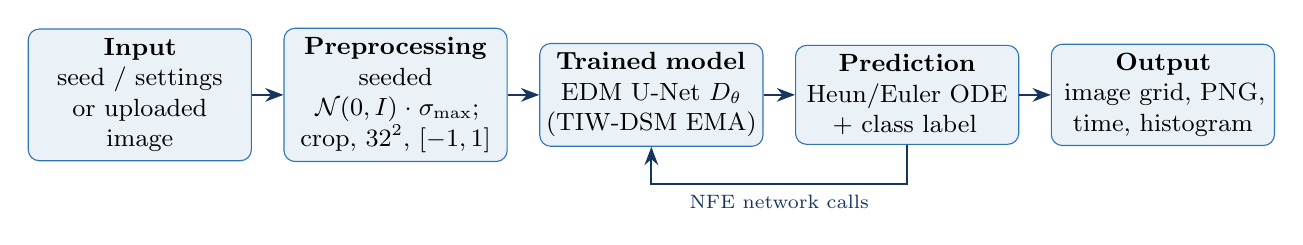
\begin{tikzpicture}[node distance=4mm, box/.style={draw=Blue,fill=PaleBlue,rounded corners,align=center,font=\small,minimum height=12mm,text width=26mm}, arr/.style={-{Stealth},thick,Navy}]
\node[box] (in) {\textbf{Input}\\ seed / settings\\ or uploaded image};
\node[box,right=of in] (pre) {\textbf{Preprocessing}\\ seeded $\mathcal{N}(0,I)\cdot\sigma_{\max}$;\\ crop, $32^2$, $[-1,1]$};
\node[box,right=of pre] (model) {\textbf{Trained model}\\ EDM U-Net $D_\theta$\\ (TIW-DSM EMA)};
\node[box,right=of model] (solve) {\textbf{Prediction}\\ Heun/Euler ODE\\ + class label};
\node[box,right=of solve] (out) {\textbf{Output}\\ image grid, PNG,\\ time, histogram};
\draw[arr] (in) -- (pre); \draw[arr] (pre) -- (model); \draw[arr] (model) -- (solve); \draw[arr] (solve) -- (out);
\draw[arr] (solve.south) -- ++(0,-5mm) -| node[pos=0.25,below,font=\scriptsize]{NFE network calls} (model.south);
\end{tikzpicture}
\caption{Deployed inference pipeline (Streamlit). The discriminator is not part of inference.}
\label{fig:pipeline}
\end{figure}
The app (\texttt{app/streamlit\_app.py}) loads only the EMA weights of the final score network. It has three tabs. \textbf{Generate} takes a seed (any integer, for example one given by the evaluator), a number of images, the solver and the step count, and can run DSM(obs) side by side on the same noise. \textbf{Image-to-image} takes \emph{any} uploaded image, preprocesses it to $32\times32$, adds noise up to a chosen strength and denoises it with the model (SDEdit \cite{meng2022sdedit}). This is a genuinely unseen input for the live demo. \textbf{How it works} explains the pipeline. The sidebar shows the checkpoint's SHA-256, its training objective, size and number of trained images. Together with the optional denoising-trajectory view, this demonstrates that outputs come from the trained model and are not stored images.

\subsection{Hosting}
The app is deployed on Streamlit Community Cloud at \appURL. The service clones the GitHub repository, installs the CPU-only dependencies in \texttt{app/requirements.txt} (PyTorch CPU wheels, NumPy, Pillow, Streamlit), loads \texttt{checkpoints/deploy/tiw\_dsm.pt} and \texttt{dsm\_obs.pt} from the repository, and serves the app publicly. Every push to \texttt{main} redeploys it. On the free CPU instance, 16 images at 35 NFE take about 10~s (about 0.6~s per image). The optional VGG13-BN class labels are shown only in local runs, where \texttt{prepare\_data.py} has exported the classifier; the hosted app omits them.

\subsection{Dependencies and local startup}
\begin{lstlisting}
pip install -r requirements.txt            # torch, numpy, scipy, pillow, streamlit, ...
mkdir -p checkpoints/deploy
# download tiw_dsm.pt (and dsm_obs.pt) from the weights link on page 1, or copy from runs/
cp runs/tiw/ema_final.pt checkpoints/deploy/tiw_dsm.pt
cp runs/obs/ema_final.pt checkpoints/deploy/dsm_obs.pt
streamlit run app/streamlit_app.py           # -> http://localhost:8501  (works offline, CPU or GPU)
\end{lstlisting}

\subsection{Input / output format}
\begin{table}[H]
\centering
\caption{Inference interface.}
\label{tab:io}
\small
\begin{tabularx}{\textwidth}{p{28mm}Y}
\toprule
Input (generate) & seed: int in $[0,2^{31})$; $n\in\{1,4,8,16,32,64\}$; solver $\in\{$heun, euler$\}$; steps $\in\{3,\dots,49\}$; model $\in\{$TIW-DSM, DSM(obs)$\}$ \\
Input (img2img) & PNG/JPG/WEBP/BMP of any size; strength $\sigma\in[0.2,20]$; noise seed \\
Preprocessing & image $k$ uses noise $\mathcal{N}(0,I)$ from \texttt{torch.Generator().manual\_seed(seed+k)}, scaled by $\sigma_{\max}=80$. Upload: centre crop, bicubic resize to $32\times32$, $x/127.5-1$, plus $\sigma\cdot$noise \\
Model output & tensor $[n,3,32,32]$ in $[-1,1]$ $\to$ uint8 $[n,32,32,3]$ \\
Displayed output & image grid (downloadable PNG), wall-clock time, ms/image, NFE, per-image class and confidence (VGG13-BN), class histogram \\
\bottomrule
\end{tabularx}
\end{table}

\subsection{Example inference (programmatic)}
\begin{lstlisting}[language=Python]
import torch
from tiwdsm.io import load_ema
from tiwdsm.edm import sample, seeded_latents
from tiwdsm.data import to_uint8
model, meta = load_ema("checkpoints/deploy/tiw_dsm.pt", "cpu")   # EMA weights only
z = seeded_latents(range(2026, 2026 + 16))                         # input: seed 2026, 16 images
imgs = to_uint8(sample(model, z, num_steps=18, solver="heun"))     # output: uint8 (16, 32, 32, 3)
\end{lstlisting}
On a Kaggle T4, generation at 35 NFE costs \resMsImg{} ms per image in batches of 500, or about 0.5~s for a single image (Table~\ref{tab:steps}). On a laptop CPU a batch of 16 images at 25 NFE takes a few seconds.

\subsection{Application screenshots}
\begin{figure}[H]
\centering
\fig{app_generate.png}{Screenshot 1: ``Generate'' tab}
\caption{Live app (\appURL), Generate tab. Seed 2026, 16 images, Heun 18 steps (35 NFE) on CPU: TIW-DSM and DSM(obs) side by side from the same noise, with wall-clock time and the denoising trajectory of the first image. The sidebar shows the loaded checkpoint (SHA-256 prefix \texttt{1366bae91a89}, objective \texttt{tiw}, 3.51 Mimg).}
\label{fig:app1}
\end{figure}
\begin{figure}[H]
\centering
\begin{minipage}{0.49\linewidth}\centering\fig{app_upload.png}{Screenshot 2: image-to-image with an uploaded photo}\end{minipage}\hfill
\begin{minipage}{0.49\linewidth}\centering\fig{app_info.png}{Screenshot 3: sidebar with checkpoint hash and model info}\end{minipage}
\caption{Left: image-to-image on an uploaded photo. Right: active-model panel (checkpoint SHA-256, objective, size).}
\label{fig:app2}
\end{figure}

% ============================================================================
\section{Limitations}\label{sec:limits}
% ============================================================================
\begin{itemize}[leftmargin=5mm,itemsep=2pt,topsep=1pt]
\item \textbf{Reduced compute.} A \resParams M-parameter network, flips instead of EDM augmentation, and 3.51 Mimg instead of 11 Mimg for the comparison. Absolute FIDs are therefore not comparable to the paper. The comparison between methods is fair: same data, architecture, training length, seeds and evaluation.
\item \textbf{One seed per model, one discriminator.} Each model was trained once and we used one discriminator checkpoint (10k iterations). The diversity loss we observe may depend strongly on that checkpoint; we could not test earlier, less confident checkpoints in the time available.
\item \textbf{Scope.} Only CIFAR-10 LT at 5\% was reproduced. CIFAR-100, FFHQ, CelebA and the other reference sizes were not. Only the DSM(obs) baseline was trained on images; IW-DSM, DSM(ref) and the W/C ablations are implemented (\texttt{--mode iw|ref}, \texttt{--no\_reweight}, \texttt{--no\_correction}) but only tested in 2-D.
\item \textbf{Measuring bias with a classifier.} The bias metric depends on a VGG13-BN trained on real CIFAR-10. Its errors on generated images, which may be off-distribution, are not corrected, and it measures only class-level bias.
\item \textbf{The reference set defines ``unbiased''.} TIW-DSM moves toward whatever $\Dref$ represents. With 500 images and a 1.63:1 spread across classes, $\Dref$ is itself a noisy target. The method cannot judge whether a target distribution is fair.
\item \textbf{Shared images.} 120 images appear in both sources. This slightly reduces the separability the discriminator can learn but was kept for fidelity to the released data.
\item \textbf{Deployment.} $32\times32$ outputs are small. Image-to-image results on arbitrary uploads are limited by CIFAR-10's ten classes and resolution.
\end{itemize}

% ============================================================================
\section{Conclusion}\label{sec:conclusion}
% ============================================================================
We reproduced TIW-DSM from our own implementation on the authors' exact CIFAR-10 LT / 5\% data. Deriving the objective in EDM's denoiser form showed that TIW-DSM is standard diffusion training with a bounded per-sample weight $2d$ and a target shifted by $\sigma^2\nabla\log d$. Our analysis and the 2-D check show that the score-correction term is what removes the bias, while weighting alone leaves the minimiser unchanged. Under a reduced but equal budget (3.51 Mimg each), the debiasing effect reproduced. TIW-DSM raised the generated tail-class share from \resTailobs\% to \resTailtiw\% (target 50\%) and lowered the Eq.~51 bias by \resBiasRed\%. The FID improvement did not: \resFIDtiw{} vs.\ \resFIDobs{}, with lower recall. Our discriminator diagnostics explain this as near-zero weights for biased images at low noise, which shrink the effective training set at exactly the noise levels that control detail and diversity. The additional experiment showed that TIW-DSM keeps its bias advantage at every budget of 17 NFE or more, that Euler is competitive with Heun for this model, and that 25 NFE is a good deployment default. Our Streamlit application uses this default to serve the trained model live on unseen seeds and uploaded images.

\textbf{Future work:} first, regularise, temperature-scale or early-stop the discriminator so that $\tilde w$ is not saturated at small $t$, and re-train TIW-DSM (the cheapest test of our explanation); then train for the full 11 Mimg, use the paper-sized \texttt{base} network with EDM augmentation, run IW-DSM and the W/C ablations on images, and test larger reference sets (10--50\%).

% ============================================================================
\section{References}\label{sec:refs}
\begingroup
\small
\renewcommand{\section}[2]{}% suppress the bibliography's own unnumbered heading
\bibliographystyle{ieeetr}
\bibliography{references}
\endgroup

\appendix
% ============================================================================
\section{Summary of Revisions from the Mid Report}\label{app:revisions}
% ============================================================================
\begin{itemize}[leftmargin=5mm,itemsep=1pt,topsep=1pt]
\item \textbf{Literature review:} condensed; added the density-ratio estimation background \cite{sugiyama2012dre}, the EDM formulation and the connection to Discriminator Guidance and ADM, which our discriminator builds on.
\item \textbf{Methodology (new):} the practical $\tilde w=2d$ form for training on $\Dobs$ (paper Eq.~36), our EDM-form derivation (Eq.~\ref{eq:edmtiw}) and the analysis of why weighting alone cannot debias (Section~\ref{sec:whyboth}).
\item \textbf{EDA:} corrected the $\Dref$ max/min ratio to 65/40 = 1.625 (the D2 notebook printed 1.62, the report 1.63). Clarified that recovered labels are used only for analysis. Added the training-time preprocessing ($\Dobs$ with 20$\times$ reference repetition, discriminator perturbation).
\item \textbf{Metrics:} added the paper's Eq.~51 bias metric, named the classifier (VGG13-BN, as in the paper), and cited and implemented recall \cite{kynkaanniemi2019pr}. In the proposal and Deliverable 2, ``35 steps'' was used loosely: 35 is the NFE of 18 Heun steps. The steps experiment now reports both.
\end{itemize}

\section{Reproducibility: exact commands}\label{app:commands}
\begin{lstlisting}
python scripts/prepare_data.py
python scripts/toy_2d.py
python scripts/train_discriminator.py --iters 10000
python scripts/train_score.py --mode obs --outdir runs/obs --duration_mimg <D>
python scripts/train_score.py --mode tiw --outdir runs/tiw --duration_mimg <D>
python scripts/evaluate.py --ckpt runs/obs/ema_final.pt --name obs --num 50000
python scripts/evaluate.py --ckpt runs/tiw/ema_final.pt --name tiw --num 50000
for r in bias ref target; do python scripts/evaluate.py --real $r --name data_$r; done
python scripts/steps_experiment.py --ckpt obs=runs/obs/ema_final.pt --ckpt tiw=runs/tiw/ema_final.pt --num 10000
python scripts/make_report_assets.py --runs obs=runs/obs tiw=runs/tiw
cd report && latexmk -pdf main.tex
\end{lstlisting}

\end{document}
